\newpage
\section{Розробка системи паралельного пошуку}
Як було показано в першому розділі існує немало програм, для пошуку у структурах гри Го, але практично всі вони є комерційними. Некомерційною є прогрма Kombilo, але вона має такі недоліки:
\begin{itemize}
	\item Складність роботи з системою. Якщо хтось захоче додати підтримку Го у свою систему, йому доведеться розбиратися з великою кількістю коду на С++.
	\item Графічний інтерфейс на Python. Хочу Python -- багатоплатформова мова, для графічного інтерфейсу краще використовувати щось більш стандарте. Наприклад одну з багатоплатформових бібліотек для С++, або щось інше.
\end{itemize}

Тому є доцільним розробити систему пошуку для гри Го, яка буде написана, використовуючи можливості Java. Це дасть змогу великій кількості людей використовувати цю систему, додавати до неї нові модулі та взагалі робити дослідження у цій області.

\subsection{Алгоритм Мінімакс}
Мінімакс -- правило прийняття рішень, що використовується в теорії ігор, теорії прийняття рішень, дослідженні операцій, статистиці і філософії для мінімізації можливих втрат з тих, які особа, яка приймає рішення не може уникнути при розвитку подій за найгіршим для неї сценарієм. Критерій мінімаксу спочатку був сформульований в теорії ігор для гри двох осіб з нульовою сумою для випадків послідовних і одночасних ходів, згодом отримав розвиток у складніших іграх і прийнятті рішень в умовах невизначеності.

Припустимо, що в грі є максимум два можливих кроки для кожного гравця на кожен хід. Алгоритм генерує дерево, де кола є ходи максимізуючого гравця, а квадрати являють собою ходи суперника (мінімізуючий гравець). Через обмеженість обчислювальних ресурсів, як описано вище, дерево обмежено на 4 кроки уперед.

\begin{figure}[H]
	\centering
	\caption{Мінімаксне дерево на 4 кроки вперед}
	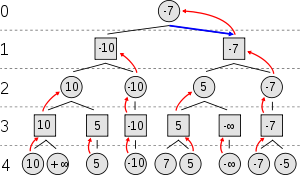
\includegraphics[width=300pt]{minimax_example}
	\label{fig:minimax_example}
\end{figure}

Мінімаксний алгоритм потребує функцію генерування можливих ходів (ходи, що не є заборонені правилами гри) та функцію еврістичної оцінки поточного стану дошки. Розробка функції оцінки стану виходить за рамки даної роботи, тому замість неї буде використовуватися випадкова величина.

Функція генерування можливих ходів (movegen у коді) використовує поточний стан дошки board та колір гравця, що робить крок player. Гравець завжди комп'ютер, але функції потрібно знати його колір, щоб вирішувати куда можно ставити камінь, адже всередину груп з однією ступінню свободи може ходити тільки гравець, чия ця група. Функція повертає список можливих ходів у вигляді пар координат. Саме ця функція має найбільші знання про гру Го. Вона повинна розуміти правило зняття з дошки каменів та правило Ко.

Алгоритм Мінімакс можно досить легко розпаралелити. Достатньо шукати максимум кожного піддерева у окремому потоці. В мові Clojure це можна легко зробити використовуючи функцію pmap. Ця функція працює як звичайний map, але запускає функції у окремих потоках, повертаючи Future. Використовуючи цей об'єкт можливо дізнатися коли закінчиться виконання відповідної функції та отримати її результат.

Така функція дозволяє досить просто розпаралелити функцію Мінімаксу, але віна не дає змогу контролювати цей процес. Якщо є така задача, то розпаралелення можна реалізувати самостійно, використовуючи ті самі об'єкти типу Future.

\begin{algorithmic}
	\Function{minimax}{node, depth}
	\Comment returns integer - value of best play
		\If {node is a terminal node \textbf{or} depth $\leq$ 0}
			\State \Return the heuristic value of node
		\EndIf
	    \State $\alpha\gets-\infty$
		\For {child \textbf{in} node}
			\Comment evaluation is identical for both players
			\State $\alpha\gets$max($\alpha$, -minimax(child, depth-1))
		\EndFor
		\State \Return $\alpha$
	\EndFunction
\end{algorithmic}

\subsection{Альфа-бета відсічення}
Альфа-бета відсічення —- алгоритм пошуку, що зменшує кількість вузлів, які необхідно оцінити в дереві пошуку мінімаксного алгоритму і при цьому дозволяє отримати ідентичний результат. Цей алгоритм використовується в програмуванні ігор, де грають два гравці (хрестики-нулики, шахи, го). Використовуючи цей алгоритм, програма повністю припиняє оцінювати хід, якщо знайшла доказ, що цей хід гарантовано гірший, ніж оцінений раніше. Такі ходи не потребують подальшого розглядання.

\begin{figure}[H]
	\centering
	\caption{Ілюстрація роботи алгоритму Альфа-бета відсічення}
	\includegraphics[width=300pt]{AB_pruning}
	\label{fig:AB_pruning}
\end{figure}

Альфа-бета алгоритм, при найкращому порядку ходів, побудує значно менше дерево перебору. Кількість вузлів приблизно дорівнює кореню квадратному з числа позицій, що переглядаються при повному переборі. Альфа-бета розподіл дуже чутливий до порядку ходів. Тому потрібно врахувати, що при найгіршому порядку ходів, тобто коли відсічення за beta розглядає останній хід, альфа-бета алгоритм прогляне стільки ж позицій, що і мінімакс. Швидкість прорахунку також дуже залежить на практиці від можливого діапазону оцінок.

Приклад псевдокоду Альфа-бета відсічення:

\begin{algorithmic}
	\Function{AlphaBeta}{color, depth, $\alpha$, $\beta$}
		\If {depth = 0}
			\State \Return \Call{Evaluate}{color}
		\EndIf
		\State moves $\gets$ \Call{GenerateMoves}{}
		\For {move \textbf{in} moves}
			\State \Call{makeMove}{move}
			\State eval $\gets$ -\Call{AlphaBeta}{-color, depth-1, -$\beta$, -$\alpha$}
			\State \Call{unmakeMove}{move}
			\If {eval $\geq \beta$}
				\State \Return $\beta$
			\EndIf
			\If {eval $> \alpha$}
				\State $\alpha \gets$ eval
				\If {depth = defaultDepth}
					\State bestmove $\gets$ move
				\EndIf
			\EndIf
		\EndFor
		\State \Return $\alpha$
	\EndFunction
\end{algorithmic}

\subsection{Порівняння з шаблоном}
Єфективне роспізнання шаблонів у грі Го та їх грамотне використання є вирішальним як для гравця-людини, так і для програми. На поточний момент було створено базу шаблонів різних етапів партії на основі професійних партій в Го. Така база використовуються майже усіма програмами, що грають у Го.

Не зважаючи на те, що велику кількість шаблонів партій з Го можна знайти в спеціалізованих базах даних, краще ці шаблони та статистику їх використання з'ясувати самим.

Спочатку дамо визначення шаблону партії Го. Шаблоном будемо називати послідовність ходів у партії, що обмежені квадратом 5x5 з першим ходом у центрі. Такий підхід дозволить швидко знаходити нові шаблони, до того ж аналізувати статистику їх використання.

\begin{figure}[H]
	\centering
	\caption{Приклад першого ходу у шаблонах в грі го}
	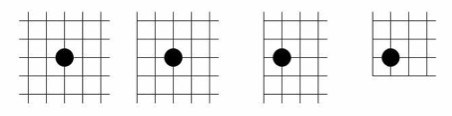
\includegraphics[width=300pt]{go_pattern_example}
	\label{fig:go_pattern_example}
\end{figure}

Також необхідно розробити метод, який би об'єднував однакові шаблони у один, з урахуванням повороту, симетрії та зміні кольору каменів на протилежний. Один із методів, що можна використати, заснований на канонічній формі шаблона.

Щоб привести шаблон до канонічної форми спочатку інвертуємо кольори ходів, якщо потрібно, щоб перший хід був чорним. Далі всього 8 варіантів перетворень можливо (4 повороти $\times$ 2 симетрії). Закодуємо кожен з цих варіантів одним числом Integer (наприклад, використовуючи Зобріст-хешування, що буде описано далі). Канонічною формою шаблону будемо називати варіант, що має найменше відповідне закодоване значення. Таким чином можливо 4 варіанти, що відображені на рис. \ref{fig:go_canonical_pattern} звести до одного.

\begin{figure}[H]
	\centering
	\caption{Приклад однакових шаблони, що повинні об'єднатися в один}
	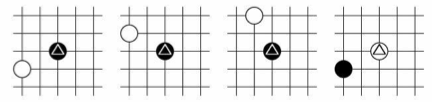
\includegraphics[width=300pt]{go_canonical_pattern}
	\label{fig:go_canonical_pattern}
\end{figure}

Далі треба створити базу шаблонів з статистичними даними, по цих зразках. Найпростіше збирати інформацію про кількість разів, яку цей шаблон був використаний у партіях, що були проаналізовані. Якщо використовувати велику кількість партій професійного рівня, то така статистика може використовуватися програмами, що грають в го, як база даних гарних ходів. Вони можут шукати частини шаблонів у іграх, а потім догравати використовуючи ті варіанти, що більш вигідні їм.

Наведемо приклад алгоритму створення подібної бази шаблонів з колекції ігор:

\begin{algorithmic}
	\For {each game record R \textbf{in} the game record collection}
		 \For {each move M \textbf{in} R}
		 	\State Play M on the game board
			\State Obtain the 5-by-5 region R centered by M
			\State Rotate and flip R into its canonical form
			\If {R is \textbf{not in} our pattern database}
				\State Add R into the pattern database
				\State Set frequency number of R to be 0
			\EndIf
			\State Increase the frequency number of R by 1
		\EndFor
	\EndFor
\end{algorithmic}

Завдяки аддитивності Зобріст-хешування пошук шаблону по такій базі дуже простий. Якщо не враховувати можливі колізії, то перевірка наявності шаблону (тобто підпослідовності ходів) у партії зводиться до виконанню операції XOR над хешом шаблону та хешом поточного стану партії. Це є дуже ефективним способом знаходення шаблонів, однак недолік полягає у тому, що таку перевірку треба робити для всіх станів дошки партії починаючи з якогось. Тобто для знаходження шаблонів у партії в 200 ходів, використовуючи базу даних з 1000 шаблонів треба виконати 200 тисяч операцій XOR.

\subsection{Зобріст хешування}
Одним із методів пошуку деякого положення каменів на дошці може будти хешування. Якщо використовувати хешування, по якому можна легко дізнатися, що стоїть на якій клітинці, то функція пошуку деякого зразка на дошці теж буде досить легкою. Прикладом такого хешування может бути Зобріст-хешування.

Зобріст-хешування -- це хеш-функція, що використовується в комп'ютерних програмах, які грають  в абстрактні настільні ігри, такі як шахи або го і використовують транспозиційні таблиці, особливий вид хеш-таблиць, що індексуються позиціями дошки і використовується, щоб уникнути аналізу однієї і тієї ж самої позиції декілька разів.

Зобріст-хешування починається з генерування випадкового бітового рядка для кожного можливого елемента настільної гри, тобто для кожної комбінації фігури і положенням (у грі в шахи, це 12 штук $\times$ 64 позицій дошки, для го, це 2 фігури $\times$ 361 позицій дошки). Тепер будь-якоа конфігурація дошки може бути розбита на незалежні компоненти фігура/положення, кожен з яких має відповідний бітовий рядок. Остаточний Зобріст хеш обчислюється через ці бітові рядки використовуючи побітовое XOR між усіма ними.

Приклад псевдокоду для гри в Го:

\begin{algorithmic}
	\State empty $\gets$ 0
	\Comment{constant figures}
	\State white\_stone $\gets$ 1
	\State black\_stone $\gets$ 2
	\Function{init\_zobrist}{}
	\Comment{fill a table of random numbers/bitstrings}
		\State table $\gets$ a 2-d array of size 361$\times$2
		\For{i \textbf{from} 1 \textbf{to} 361}
		\Comment{loop over the board, as a linear array}
			\For{j \textbf{from} 1 \textbf{to} 2}
			\Comment{loop over the figures}
				\State table[i][j] $\gets$ \Call{random\_bitstring}{}
			\EndFor
		\EndFor
	\EndFunction
	\Function{hash}{board}
		\State h $\gets$ 0
		\For{i \textbf{from} 1 \textbf{to} 361}
		\Comment{loop over the board positions}
			\If{board[i] $\neq$ empty}
				\State j $\gets$ the piece at board[i], as listed in the constant figures, above
				\State h $\gets$ h XOR table[i][j]
			\EndIf
		\EndFor
		\State \Return h
	\EndFunction
\end{algorithmic}

\subsection{Метод Монте-Карло}
Метод Монте-Карло -- загальна назва групи числових методів, основаних на одержанні великої кількості реалізацій стохастичного (випадкового) процесу, який формується у той спосіб, щоб його ймовірнісні характеристики збігалися з аналогічними величинами задачі, яку потрібно розв'язати. Використовується для розв'язування задач у фізиці, математиці, економіці, оптимізації, теорії управління тощо.

Метод Монте-Карло — це метод імітації для приблизного відтворення реальних явищ. Він об'єднує аналіз чутливості (сприйнятливості) і аналіз розподілу ймовірностей вхідних змінних. Цей метод дає змогу побудувати модель, мінімізуючи дані, а також максимізувати значення даних, які використовуються в моделі. Побудова моделі починається з визначення функціональних залежностей у реальній системі. Після чого можна одержати кількісний розв'язок, використовуючи теорію ймовірності й таблиці випадкових чисел.

Для пошуку гри в Го існує метод Монте-Карло пошуку по деревах. Він генерує велику кількість випадкових партій до кінця гри. Потім він рахує статистику виграшу та програшу у цих іграх. Використовуючи цю статистику, він приймає рішення щодо наступного ходу, вибираючи хід, що має найбільшу вірогідність виграшу.

Цей метод потребує розширення структури дерева варіантів гри. Він додає 2 значення у кожний вузол: статистику виграшів ($winrate \in [0; 1]$) та число раз, що цей вузол був відвіданий. На основі цих двох значень використовуючи функцію, показану нижче, алгоритм вираховує найкращий шлях для продовження аналізу на початку кожного кроку.

\begin{equation*}
    UCTValue(parent,n)=winrate+\sqrt{\frac{\ln(parent.visits)}{5\times n.nodevisits}}
\end{equation*}

Алгоритм має таку структуру:
\begin{itemize}
	\item Вибір найкращого можливого маршруту
	\item Продовження кінцевого вузла випадковим чином
	\item Симуляція великої кількості випадкових ігор
	\item Оновлення значень в усіх пройдених вузлах
	\item Повторення з початку
\end{itemize}

\subsection{Обробка SGF-файлів}
Smart Game Format (SGF) -- комп'ютерний формат даних, що зберігає партії ігор, таких як Го, шахи, шашки та реверсі. Це простий, текстовий формат, що зберігає партії у вигляді дерев.

Були розроблені функції, що дозволяють маніпулювати цим файлом: читати його, перетворювати у внутрішній формат, спрощувати дерево, перетворювати у формат, що відображає положення дошки, та вивід цієї дошки на монітор.

Читання та перетворення SGF-файлу запрограмовано у вигляді лексеру та парсеру. Лексер має на вході послідовність символів з файлу, що читаються по мірі необхідності, а генерує послідовність лексем. Тобто ключових слів, що притаманні данному формату.

Список реалізованих лексем:
\begin{itemize}
	\item :treestart
	\item :treeend
	\item :nodestart
	\item :propvalue
	\item :propvalueend
	\item :propident
\end{itemize}

Далі використовується функція, що парсить список лексем, генеруючи дерева властивостей. Саме ця функція повинна знати граматичні правила даного формату.

Найчастіше для пошуку потрібні тільки ті властивості у дереві гри, що відповідають позиціям каменів гравців, усі ж інші властивості -- зайві. Тому була реалізована функція simplify, що фільтрує та спрощує дерево гри, залішаючи тільки послідовність ходів гравців. З такою структурою даних набагато легше працювати, до того ж вона займає менше пам'яті комп'ютера.

Досить часто доцільніше використовувати іншу структуру даних, що репрезентує поточний стан дошки. Ця структура вже не дерево, вона має вигляд матриці значень клітинок дошки (тобто ця клітинка пуста, зайнята білим каменем, або зайнята чорним каменем). Ця структура більш зручна, якщо треба аналізувати поточний стан дошки, адже дерево не має у собі таку інформацію. Ця структура даних необхідна для методу пошуку шаблону, саме на її основі рахується хеш поточного стану дошки.

Для візуалізації поточного стану дошки використовується функція print-board, що виводить на монітор дошку з каменями гравців. Вивід цієї функції схожий на вивід дошки у програмі GnuGo.

\begin{figure}[H]
	\centering
	\caption{Приклад виводу функції print-board}
	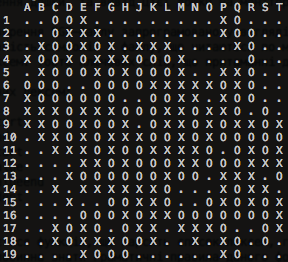
\includegraphics[width=230pt]{print-board}
	\label{fig:print-board}
\end{figure}
